\documentclass[twocolumn]{jsarticle}
\usepackage[dvipdfmx]{graphicx}
\usepackage{kenzemi}
\usepackage{amsmath}
\usepackage{nidanfloat}

\begin{document}

\title{電圧制限回路の設計と動作概要}
\author{藤田 誉大}
\date{2019年9月30日}
\abstract{既設計回路における問題点に対処する回路を提案する.ダイオードを用いた電圧制限回路を実装することにより,VCO(電圧制御発振器)の非線形性に起因する問題を排除する.新規設計回路についてLTspiceによりシミュレーションを行い,その動作を確認する.(123)}
\keyword{FSK,SWIPT,電圧制限回路}
\maketitle

\section{はじめに}
夏季休暇においては,春学期に設計したFSK-SWIPTシステムの動作確認を行ったものの,所望の動作は実現できなかった.前回の報告でその原因と改良指針について述べたが,今週はそれに基づいて新たな回路の設計を行ったため,設計回路の概要について述べる.

\section{改良回路の概要}
前回の報告で述べた既設計回路の問題点は, 1. 半固定抵抗の選定が不適当であったため,PLLの出力周波数範囲を制限できない 2. VCOの制御電圧を制限していなかったことにより,PLLのロック不良が生じる  という点であった.うち前者については,部品の再選定以外の改良は行っておらず特筆すべきことはないため,以下後者について述べる.\par 
図1に,改良部を含むPLLの周辺回路図を示す.同図において,赤点線内が新たに付加した回路である.半固定抵抗$R_5,R_6$により得られる電源電圧$V_{DD}$の分圧を$V_x, V_y (V_x<V_y)$とし,ダイオード$D_1,D_2$がそれぞれ理想的な特性であると仮定すると,LPFの出力電圧$V_{LPF}$は$V_x<V_{LPF}<V_y$の範囲に制限される.これは,$V_{LPF}<V_x$でダイオード$D_1$が,$V_{LPF}>V_y$でダイオード$D_2$がそれぞれ導通するためである.実際には,制限される電圧の範囲はダイオードの順方向電圧降下$V_F$などに影響されるため,半固定抵抗$R_5,R_6$を可変することにより実験的に調整する.その他,LPFの時定数を可変できるよう抵抗$R_1,R_2$を半固定としたほか,将来的にLPFをラグ・リードフィルタに換装することを想定し,抵抗$R_3$とキャパシタを$C_2$を付加できるようにするなど,細かい改良を施している.ラグ・リードフィルタは,それぞれ2つずつの抵抗器とキャパシタで構成されるフィルタで,高域で位相が戻る特性を持ち大きな位相余裕を確保できることから,PLLのループフィルタとして広く用いられているものである\cite{Enzaka2014}.なお参考として,改良部を含む全体の回路図を図2に示す.\par
図3,図4に,電圧制限回路のシミュレーション回路とその結果をそれぞれ示す.図4上側が入力波形で,1秒間で$0-5 \, \mathrm{[V]}$に変化するランプ波である.下側は出力波形で,おおよそ$1-4 \, \mathrm{[V]}$の範囲に電圧が制限されていることが分かる.

\section{おわりに}
今週は,前回の報告で述べた既設計回路における問題点に対処する回路の設計を行った.すでに基板レイアウトまで完了しているため,早期の発注・実装を目指したい.また,基板が到着するまでの時間を利用して,オペアンプコンテストに向けた設計や,デモ用の大型コイルについての検討を行いたいと考えている.

\begin{figure*}[b]
\begin{center}

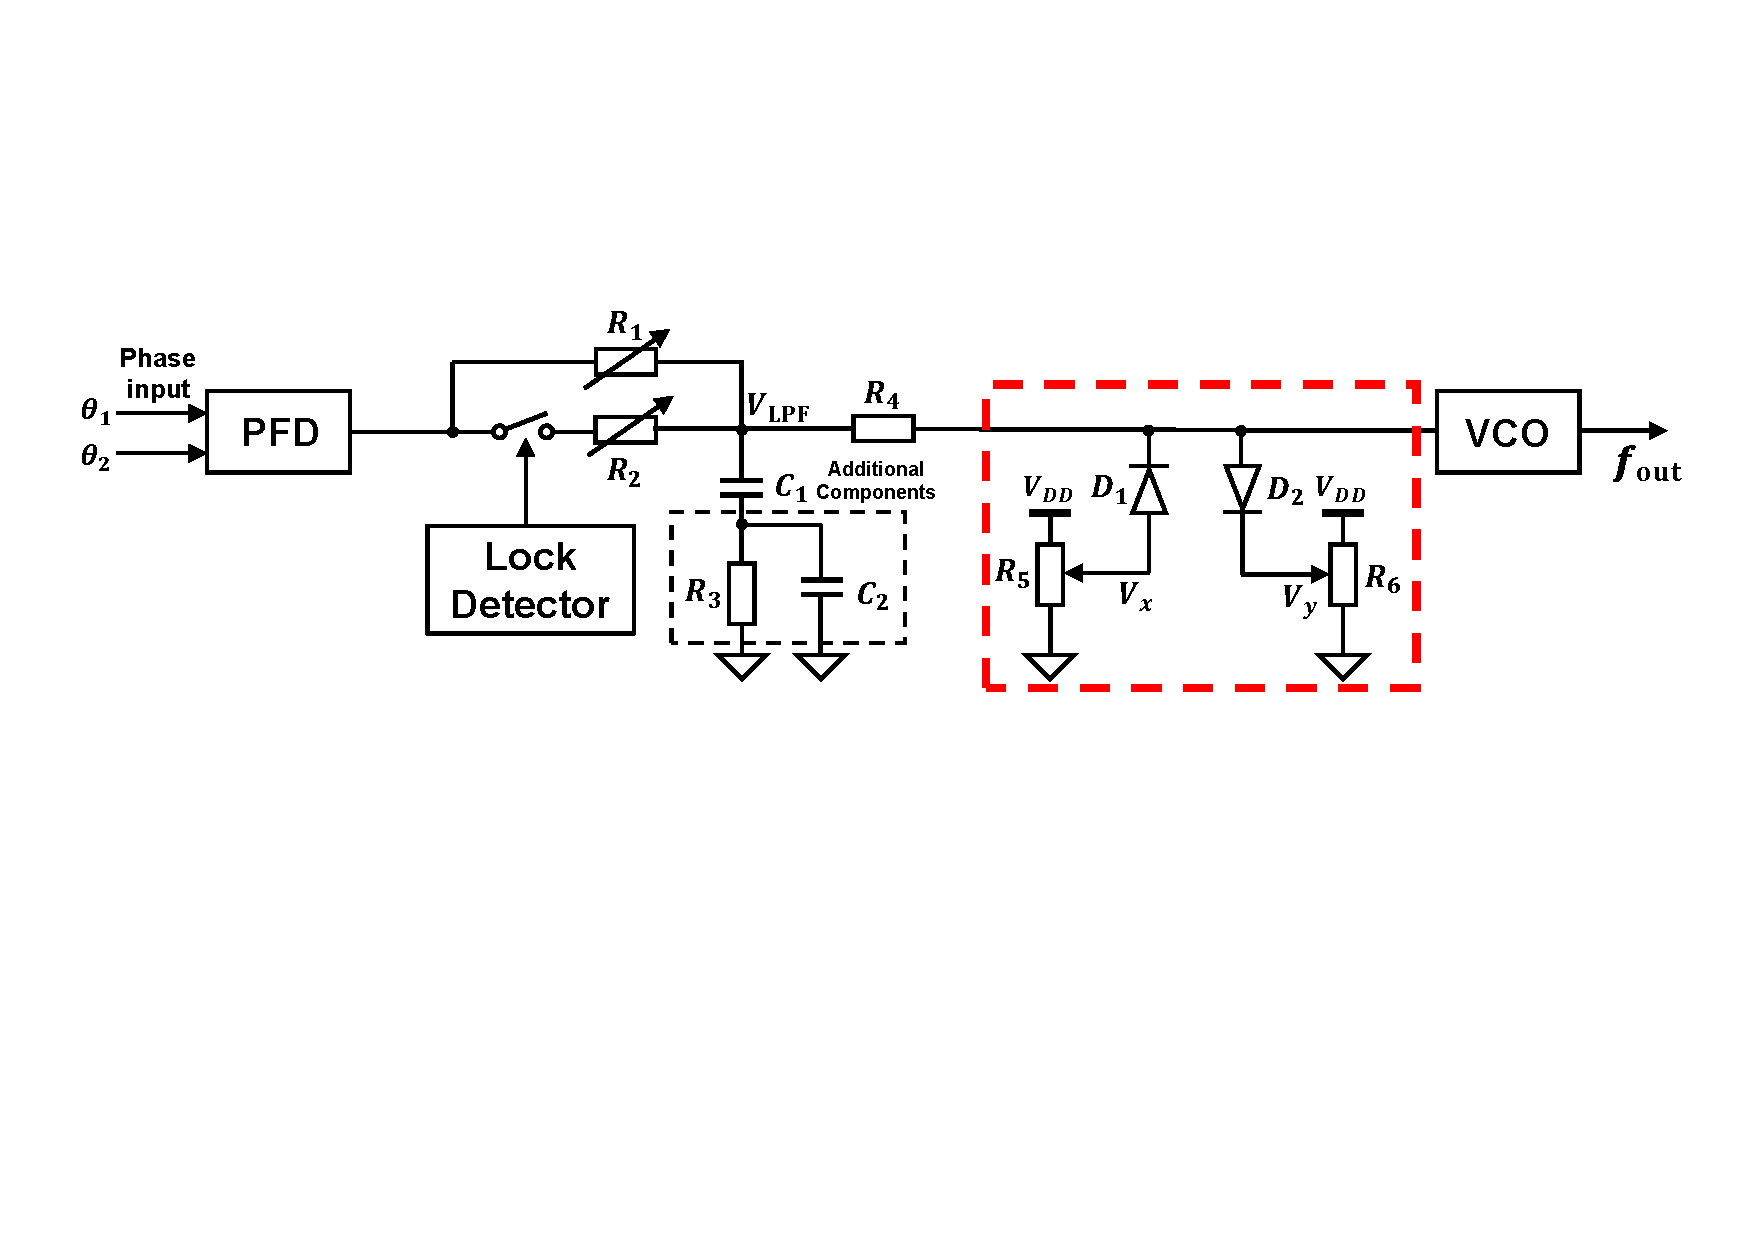
\includegraphics[width=160mm]{figures/1.pdf}
\caption{改良回路}

\end{center}
\end{figure*}

\begin{figure*}[p]
\begin{center}

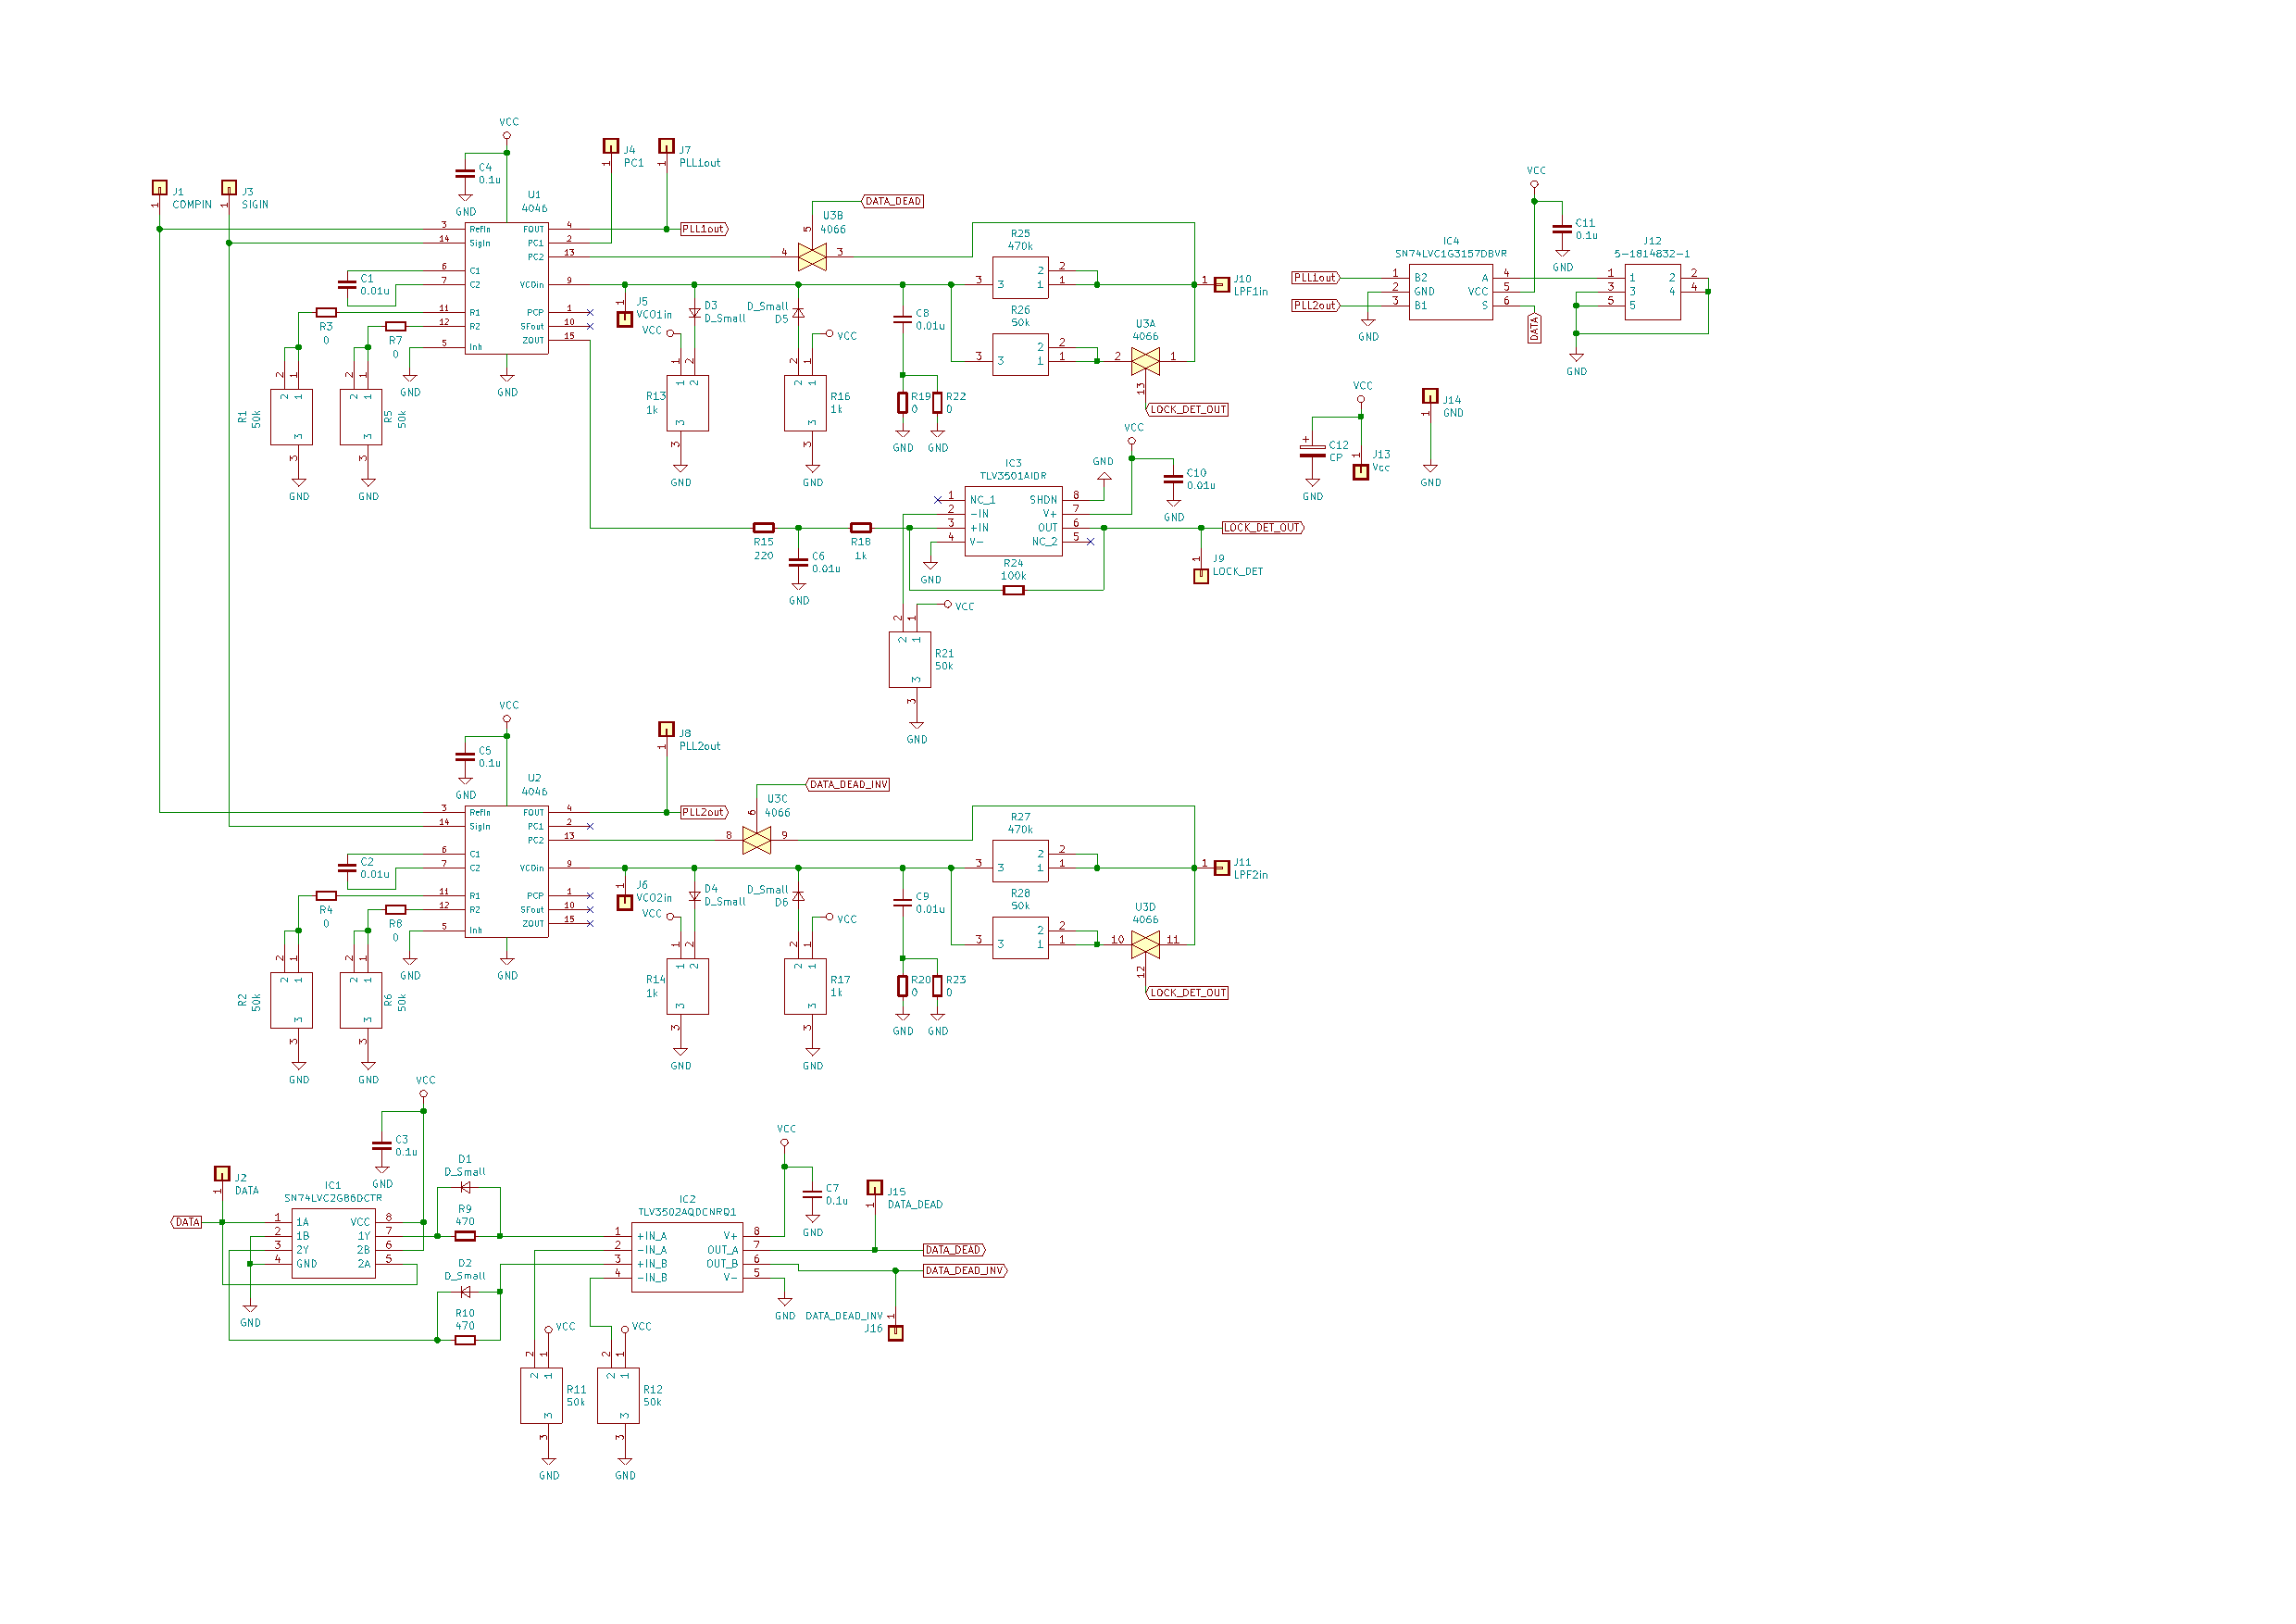
\includegraphics[width=180mm]{figures/wpf12_circuit.pdf}
\caption{改良回路の全体図}

\end{center}
\end{figure*}
\begin{figure*}[p]
\begin{center}

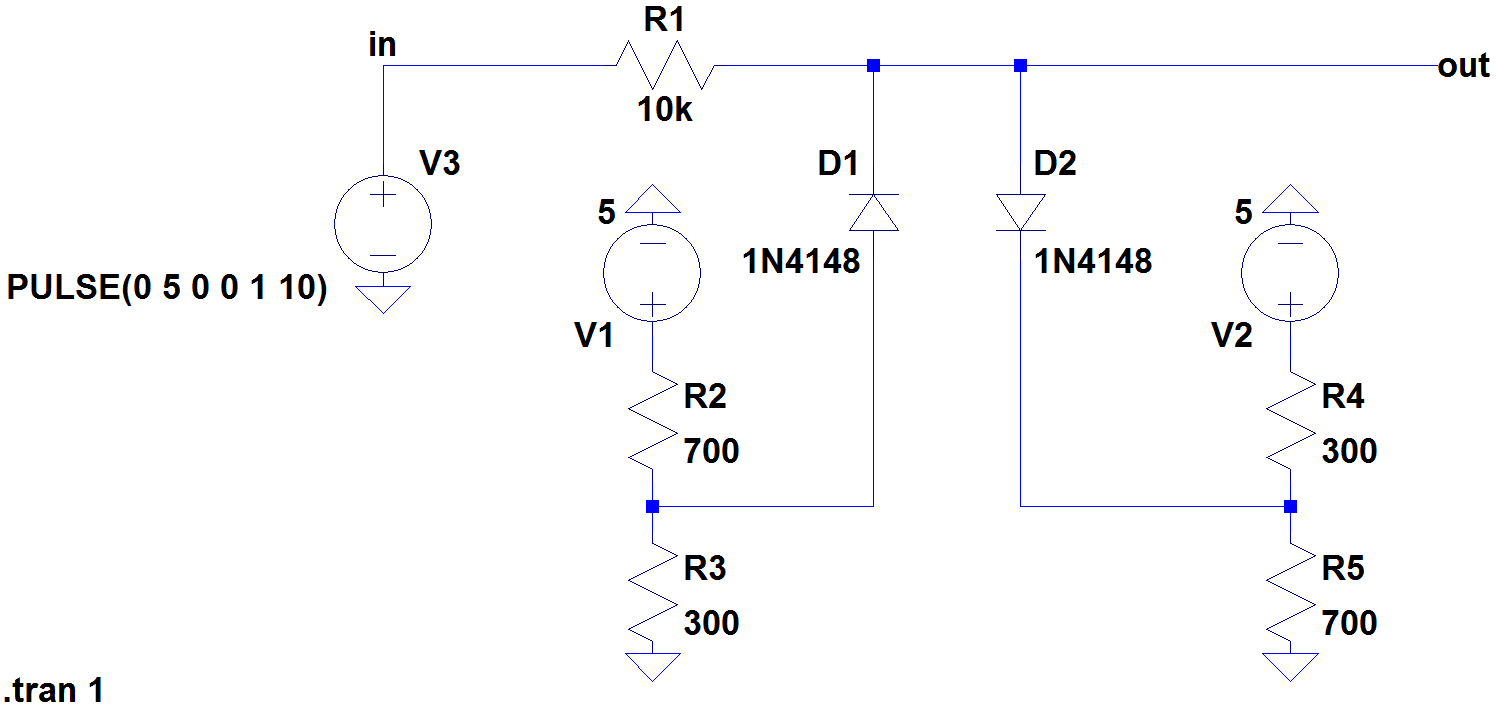
\includegraphics[width=160mm]{figures/circuit.png}
\caption{シミュレーション回路}

\vspace{1cm}
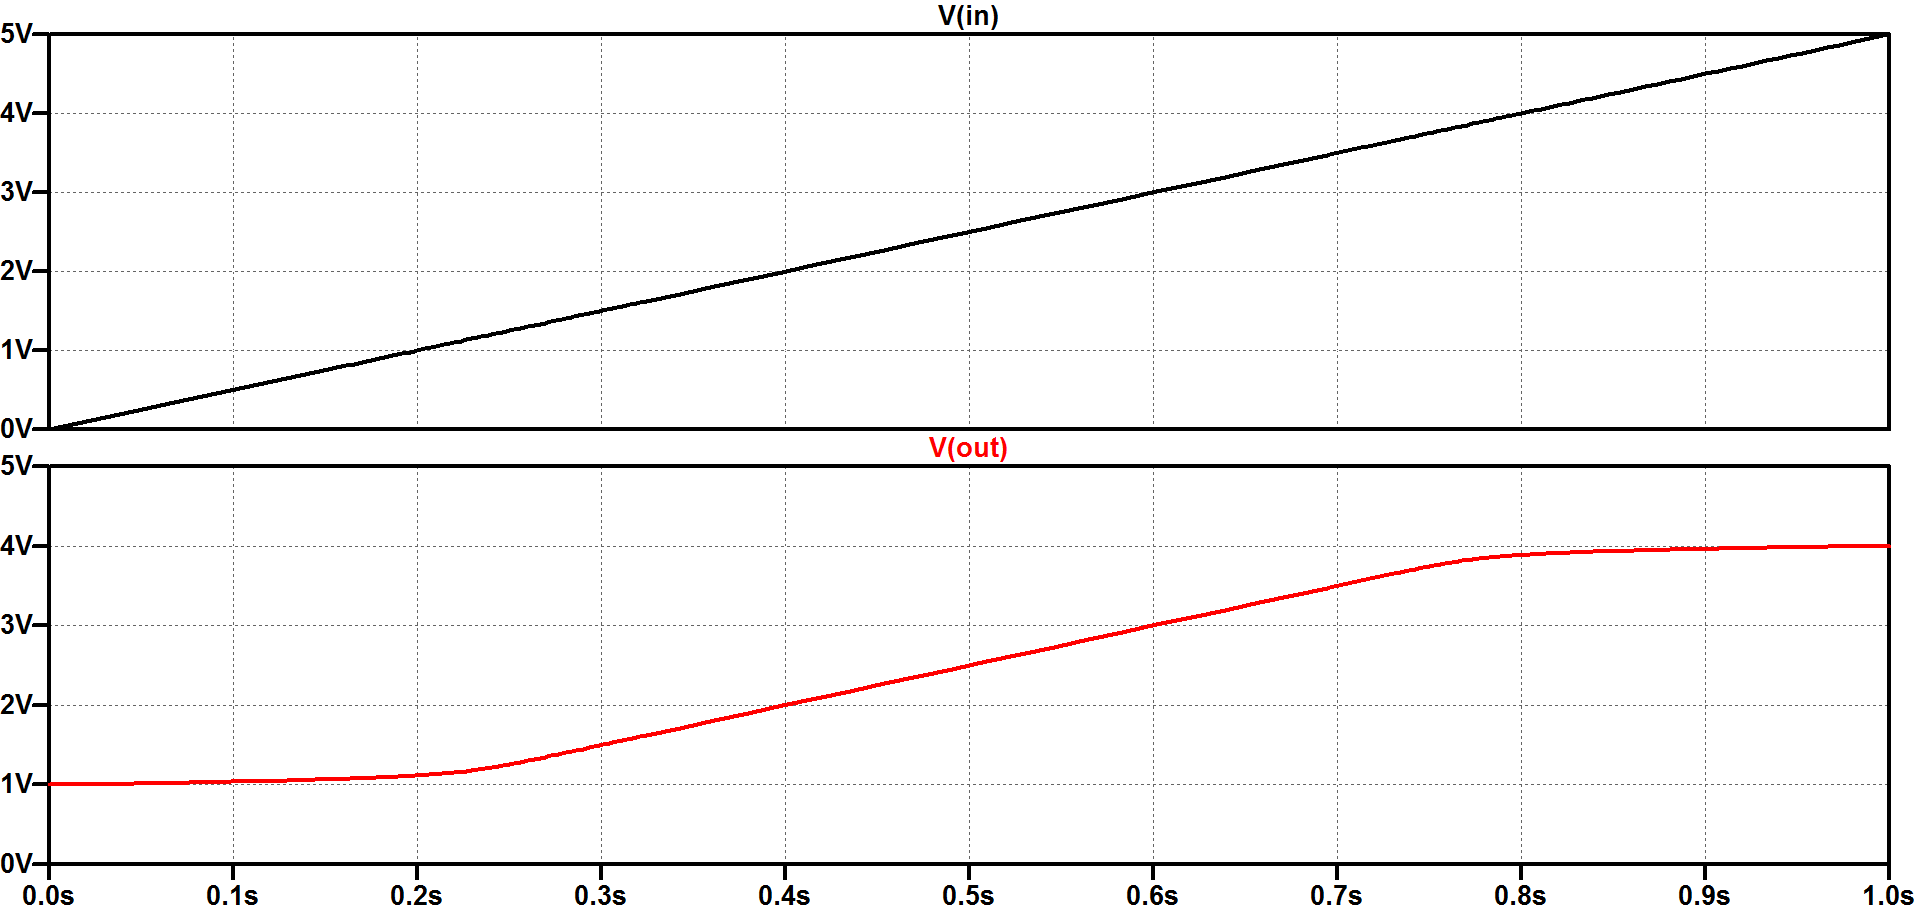
\includegraphics[width=160mm]{figures/result.png}
\caption{シミュレーション回路}

\end{center}
\end{figure*}


\begin{thebibliography}{9}
\bibitem{Enzaka2014} 遠坂俊昭, PLL回路の設計と応用, CQ出版, 2014.
\end{thebibliography}

\end{document}

